\documentclass{article}
\usepackage[final,nonatbib]{neurips_2019}
\usepackage[utf8]{inputenc}
\usepackage[T1]{fontenc}
\usepackage{amsmath,amssymb,booktabs,graphicx,microtype,float}
\usepackage[hidelinks]{hyperref}
\hypersetup{pdftitle={Can Consistent Forces Recover Molecular Shapes?},pdfauthor={Shedrack Eze; Olufunke Abodunrin; Emmanuel Aaron; Muhammed Idris}}
\makeatletter
\renewcommand{\@noticestring}{11-785 Introduction to Deep Learning, Fall 2026. Group 9 midterm working draft, 21 October 2026.}
\makeatother
\title{Can Consistent Forces Recover Molecular Shapes?}
\author{Shedrack Eze (seze) \quad Olufunke Abodunrin (oabodunr)\\
\textbf{Emmanuel Aaron (eaaron) \quad Muhammed Idris (midris)}\\
Carnegie Mellon University \quad Group 9, Path 3}
\newcommand{\funit}{\mathrm{meV}/\text{\AA}}
\begin{document}
\maketitle
\begin{abstract}
A molecule is a group of atoms, the tiny pieces of matter, and its shape is their arrangement in three dimensions. Forces push and pull these atoms, so learned force predictions can guide a computer search for a stable shape. Energy is a number associated with an arrangement, and energy-derived models calculate forces from its negative slopes, which describe how that number changes as atoms move. Direct models predict the force arrows themselves, while consistency training penalizes disagreement with the energy-derived arrows.

We compare these approaches at similar force error and computing cost on aspirin, using validation examples reserved for model selection. Direct and consistency models meet our matching rule at one consistency strength, but all five tested models recover zero of ten targets. This failure includes the energy-derived comparison model, even though all target shapes appear in training, so the pilot cannot rank successful recovery. Inaccurate forces at reference shapes and excessive coordinate steps leave the recovery question open.
\end{abstract}
\section{Why this problem matters}
Repeated physics calculations can make molecular simulation expensive, so a learned model offers a faster approximation. Training changes its adjustable numbers, called parameters, to reduce prediction errors against reference examples.

Energy is a number associated with an atomic arrangement, similar to how changing a stretched spring changes its stored energy and pull. Energy slope means how quickly that energy changes when an atom moves, and an energy-derived model calculates force arrows from the negative slopes. A direct-force model predicts the arrows themselves, while our consistency training penalizes disagreement between those arrows and forces calculated from negative energy slopes.

Our objective is to compare correct-shape recovery at similar force error and measured computing cost. Recovery requires the search to reach its assigned target shape and meet the force stopping rule; neither condition alone establishes success.
\section{What earlier studies establish}
Landscape17 supplies molecular shapes, reference forces and paths between stable arrangements~\cite{landscape}. It motivates checking final shapes beyond prediction errors, while Bigi et al. describe problems when direct forces do not follow one energy function~\cite{bigi}. Together, these studies motivate separating a force-based stop from structural success.

We build our models with E3x, software for networks that obey three-dimensional symmetry rules~\cite{e3x}. MACE supplies a separate established model for predicting energies and forces~\cite{mace}. Earlier work already studies physical constraints in training losses~\cite{takamoto}. We compare error, cost and recovery under shared conditions; consistency training itself is not new.

\section{Data and a fair comparison}
We use aspirin from Landscape17~\cite{landscape}, with 21 atoms in each molecule. Reference energies and forces come from hybrid density-functional theory, a detailed calculation based on electron physics, so these reference labels are calculated answers rather than exact experimental truth.

A transition state is a high-energy arrangement with two downhill branches toward stable arrangements, called minima. A connection group contains both branches' records, which stay in the same partition to avoid separating the two sides of one transition state. Training adjusts parameters, validation selects settings and saved models, and the test partition is reserved for later trained-model evaluation.

Training/validation/test contain 26/5/6 connections and 4,891/974/1,127 records. Training-only normalization puts energy and force errors on comparable scales, while shared minima mean that records are not independent examples of new destinations. Empirical branch classifications corrected 26 of 74 targets previously assigned from filename ordering. Earlier model-free software checks parsed test coordinates and labels, but no trained test scoring has occurred.
\subsection{Inputs, outputs and the three model types}
Our E3x models are graph neural networks in which atoms are nodes and nearby atom pairs form links. Successive calculation stages, called layers, pass learned information along these links. Inputs are atom types and three-dimensional positions; outputs are one molecular energy and a force arrow for each atom. All arms use 64 feature channels containing learned numbers and vectors, with two interactions passing messages and eight radial functions describing pair distances.

Links extend to 5~\AA, where an angstrom (\AA) is $10^{-10}$ metres. Internal features carry scalar numbers and vectors with direction. Rotating a molecule rotates its predicted forces without changing its energy, properties called equivariance for forces and invariance for energy. The energy model has 43,521 parameters; models with separate energy and force outputs have 43,649.

Our baseline, the energy comparison model, calculates $\widehat{\mathbf F}^{E}=-\nabla_{\mathbf R}\widehat E$. Here, $\widehat E$ is predicted energy, $\mathbf R$ contains atom positions, and the gradient gives energy slopes along position coordinates. Both direct arms also predict energy trained against reference labels, so they are not force-only models. Ordinary direct training has no agreement penalty, while consistency training adds one.
\subsection{Training loss and measured success}
The loss combines normalized squared energy error, normalized squared force error and, where applicable, force--energy disagreement; training adjusts parameters to reduce this number:
\begin{equation}
\mathcal L=w_E\,\mathrm{mean}(e_E^2)+w_F\,\mathrm{mean}(e_F^2)
+\lambda\,\mathrm{mean}\!\left[\left((\widehat{\mathbf F}^{D}-\widehat{\mathbf F}^{E})/s_F\right)^2\right].
\end{equation}
Here, $e_E$ and $e_F$ are prediction errors divided by their training-derived scales, with $s_F$ denoting the force scale. The superscript $D$ means directly predicted force. Weights $w_E=0.014584365670390719$ and $w_F=1.9854156343296092$ balance supervised errors. The energy baseline omits the final term, while direct training uses $\lambda=0$ and consistency training uses a positive $\lambda$.

Final E3x fits use Adam to update parameters, learning rate 0.003 and 64-bit floating-point arithmetic. Each update samples four records that can repeat, giving 800,000 sampled exposures across 200,000 updates. Two seeds, specifying random initialization and sampling, partly check repeatability.

Validation occurs every 500 updates, including zero, and BEST is the first saved model state, or checkpoint, with minimum validation force error.

Our main score, force mean absolute error (MAE), averages mistakes without their signs across the three coordinate directions of each force arrow. We give each validation connection equal weight, and smaller values are better.

Scores use meV/\AA: a millielectronvolt is one thousandth of an electronvolt, an energy unit, and energy divided by distance measures force.

Recovery additionally requires maximum predicted force component $\leq0.01$~eV/\AA\ and aligned structural RMSD $\leq0.05$~\AA. Root-mean-square deviation (RMSD) measures typical atom-position disagreement after rotation, translation and allowed atom-symmetry matching. Small predicted force is a stopping condition; it is not small prediction error.

\section{What we trained and learned}
\subsection{A fitting plateau changed the training recipe}
Early small-subset checks plateaued, but MACE Run B fitted the same 128 frames and reduced force squared error to 0.001515 of predicting zero. Different settings prevent a controlled comparison, but the plateau did not establish an unavoidable data or energy-derived-force limit.

Later 1,000-update energy and direct fits selected update zero as BEST: training improved energy but worsened force predictions.

We then completed three 200,000-update energy baselines (Figure~\ref{fig:baseline}). A used width 32 and learning rate 0.001; B used width 64 and 0.003. Both used equal normalized energy/force weights, while C retained B's structure and rate but used the balanced weights in Section 3.2. Width counts internal feature channels.
\begin{figure}[H]
\centering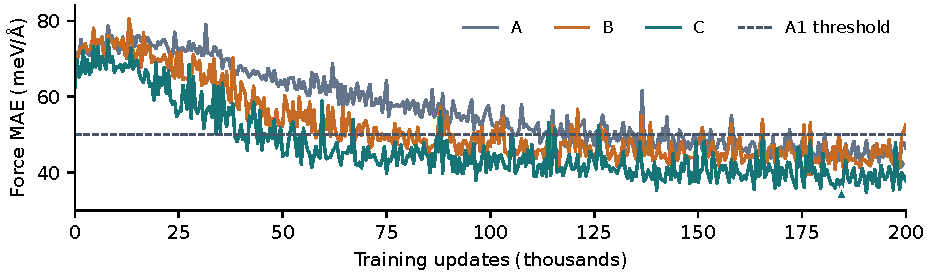
\includegraphics[width=0.85\linewidth]{figures/baseline-curves.pdf}
\caption{Our energy-baseline validation results. Lower force MAE is better. Markers show BEST; the dashed line is the declared 50~meV/\AA\ adequacy rule. Each point uses all 974 validation records, with equal connection weighting.}\label{fig:baseline}
\end{figure}
C reached 34.587~meV/\AA, versus 40.370 for B and 42.108 for A, and passed the adequacy rule. Predicting zero force gives 62.504~meV/\AA, so C reduces that error by 44.664\%. However, C's energy error is higher than B's: 126.990 versus 28.178~meV per molecule. We selected C on the energy model and transferred its recipe without retuning the other model types.
\subsection{Agreement improves, but recovery still needs a separate test}
We reused C seed zero and trained nine more fits, giving two seeds per row in Table~\ref{tab:prediction}. Consistency strength 0.1 reduces normalized force--energy disagreement squared error to 0.49--0.61, versus 116--379 for direct training. Its measured fit-plus-score time is 1.985 times direct prediction, excluding other diagnostics and overhead. This is not inference speed.
\begin{table}[H]
\centering\small
\caption{Validation error at BEST. Force columns use meV/\AA; energy uses meV per molecule. Seed limits show two observed values, not confidence bounds.}\label{tab:prediction}
\begin{tabular}{lrrr}\toprule
Model & Mean force MAE & Seed min--max & Mean energy MAE\\\midrule
Energy-derived & 34.893 & 34.587--35.198 & 128.725\\
Direct & 38.186 & 37.291--39.082 & 76.684\\
Consistency $\lambda=0.1$ & 38.024 & 36.773--39.275 & 87.006\\
Consistency $\lambda=1$ & 34.683 & 33.723--35.643 & 112.341\\
Consistency $\lambda=10$ & 39.725 & 39.060--40.390 & 161.662\\\bottomrule
\end{tabular}
\end{table}
Only strength 0.1 meets our declared matching rule against direct prediction: the mean-error gap must be within 10\% of the smaller mean and within both seed spans. A span is maximum minus minimum.

BEST is optimistic because it selects among 401 checks, while late baseline errors vary by 2.2--3.1~meV/\AA\ standard deviation across correlated checks. Nine subsequent fits finish 0.1--7.4~meV/\AA\ above BEST, and the 0.162~meV/\AA\ matching gap is smaller than this variation. Matching does not establish equivalence.

MACE Run A independently scores 5.349~meV/\AA\ with equal connection weighting after 2,048 epochs, or training-data passes. Architecture, exposure and hardware differ; this is an external reference, not a controlled efficiency comparison. MACE recovery remains unmeasured.

\section{The shape-search pilot fails for every evaluated checkpoint}
A relaxation procedure repeatedly moves atoms along predicted forces, and we tested five saved E3x checkpoints from the same ten branch starts across five validation connections. Each branch has its own target, and all six distinct target minima appear in training. Leaving the starts unchanged recovers zero targets, while every evaluated checkpoint also recovers 0/10 (Table~\ref{tab:recovery}). This fails our recovery pilot gate, so successful recovery cannot rank the methods.

The procedure proposes $\mathbf R_{\mathrm{trial}}=\mathbf R+\eta\widehat{\mathbf F}$, where $\eta$ converts predicted forces into coordinate changes. It starts at 0.2~\AA$^2$/eV and can grow to 1.0. Backtracking halves a failed trial's scale; each branch permits 1,500 force attempts.

The procedure checks force convergence first; otherwise, forces pointing broadly in compatible directions can permit acceptance. There is no energy-decrease test or per-atom movement cap, so a scale limit does not cap movement when forces are large.
\begin{table}[H]
\centering\small
\caption{All checkpoints recover 0/10 original targets. ``Wrong stop'' meets the predicted-force rule but misses the target shape. Reference-start controls begin at the six target minima; they are separate follow-up checks, called post-hoc analyses.}\label{tab:recovery}
\begin{tabular}{lrrr}\toprule
Checkpoint & Wrong stop & No convergence & Reference-start recovery\\\midrule
Energy C, seed 0 & 2 & 8 & 4/6\\
Direct, seed 0 & 4 & 6 & 1/6\\
Direct, seed 1 & 4 & 6 & 0/6\\
Consistency 0.1, seed 0 & 6 & 4 & 0/6\\
Consistency 0.1, seed 1 & 9 & 1 & 0/6\\\bottomrule
\end{tabular}
\end{table}
Across 50 model/branch outcomes, 25 stop with wrong geometry and 25 fail to converge. Reusing the same five connections does not create 50 independent paths. The reference-start controls favour the energy checkpoint under this procedure, but do not isolate a consistency-penalty effect.
\subsection{Why a small predicted force can be misleading}
A 155-evaluation check reproduced all 50 stopping flags. Every model exceeds the stopping force threshold at all 11 exact reference minima, although the reference labels themselves stay below 2.745~meV/\AA. This mismatch at exact reference shapes does not exclude nearby shapes meeting both tolerances.

All 23 force-converged direct/consistency endpoints have disconnected 5~\AA\ neighbour graphs, with atoms in different fragments beyond the model's interaction cutoff. These are not intact molecular shapes, although internal fragment forces can remain. Only seven endpoints have every atom isolated, where the direct model predicts exactly zero force automatically; this does not establish a correct molecular minimum.

Four selected trace replays reproduced the saved endpoints. Two separated, with largest accepted atom movements of 436.721~\AA\ for direct prediction and 268.047~\AA\ for energy-derived forces. The other two remained connected, with maxima 0.086492~\AA\ for consistency and 0.006083~\AA\ for energy-derived forces. Both force-converged energy endpoints remain connected.

These observations expose model and procedure limitations without proving that the procedure alone caused the failures or that real molecular break-up occurred. No evaluated E3x model recovers an original target under this procedure, and better agreement on stored examples does not establish agreement everywhere or guarantee correct shapes. Zero recovery cannot establish method equivalence.

Evidence covers aspirin, five validation connections and two seeds, with shared minima. Validation selects settings and BEST; test generalization is unestablished. Failed and incomplete trials remain recorded.

\section{A related representation check and the remaining work}
Faculty feedback prompted four new scalar-only fits and reuse of two completed scalar-and-vector E64 fits. Scalars carry numbers and vectors also carry direction, but all models still predict forces that rotate correctly with the molecule. E64 had lower validation error under its own fixed training recipe in both seeds, but this preliminary observation does not isolate a feature-type effect or establish recovery improvement. Independent interpretation review remains pending, and full results are in the companion evidence.

\paragraph{Changes from the proposal.}
We completed two seeds rather than the proposed three, and paracetamol replication is deferred until aspirin recovery is feasible. A revised adequacy protocol followed the preserved small-subset failures; responsibilities changed, and the representation check adds an extension. Long-range interactions beyond 7~\AA\ remain future work, not an explanation established by these results.
\paragraph{Three next actions.}
First, finish the MACE loader, check its predictions against saved validation outputs, and run the unchanged ten-start and six-reference controls. Second, use that evidence to assess a separately declared procedure with a per-atom movement cap, comparing the same checkpoints and starts and labelling reused-validation analysis as a post-hoc follow-up.

Third, measure closed-loop work and prediction time on identical hardware, declaring any matched-wall-time training budget before new runs. Closed-loop work totals force along a path returning to its start and checks energy consistency.
\paragraph{Team contributions and reproducibility.}
Shedrack completed data preparation, model/training integration, the first MACE reference and current experiments, while Olufunke authored the recovery evaluator. Emmanuel Aaron owns remaining physical/cost analysis, and Muhammed Idris owns MACE loading, prediction checks and independent reproduction.

Assignments are not completed contributions. Code/evidence: \href{https://github.com/Shedrackeze002/idl-molecular-force-consistency/pull/10}{GitHub PR \#10}, stacked on PRs \#9 and \#8. Before submission, confirm contributions, staff access to this private repository, live course instructions and final team approval.
\begin{thebibliography}{5}\small
\bibitem{landscape} V. C\u{a}rare et al. Global properties of the energy landscape: a testing and training arena for machine learned potentials. \emph{npj Computational Materials}, 12:9, 2026. \href{https://doi.org/10.1038/s41524-025-01878-x}{doi:10.1038/s41524-025-01878-x}.
\bibitem{bigi} F. Bigi, M. F. Langer and M. Ceriotti. The dark side of the forces: assessing non-conservative force models for atomistic machine learning. \emph{ICML}, PMLR 267:4384--4414, 2025. \url{https://proceedings.mlr.press/v267/bigi25a.html}.
\bibitem{e3x} O. T. Unke and H. Maennel. E3x: E(3)-equivariant deep learning made easy. arXiv:2401.07595, 2024. \url{https://arxiv.org/abs/2401.07595}.
\bibitem{mace} I. Batatia et al. MACE: Higher order equivariant message passing neural networks for fast and accurate force fields. \emph{NeurIPS}, 35:11423--11436, 2022. \url{https://arxiv.org/abs/2206.07697}.
\bibitem{takamoto} M. Takamoto, V. Zaverkin and M. Niepert. Physics-informed weakly supervised learning for interatomic potentials. \emph{ICML}, PMLR 267:58282--58310, 2025. \url{https://proceedings.mlr.press/v267/takamoto25a.html}.
\end{thebibliography}
\end{document}
